\documentclass[a4paper,]{article}
\usepackage[left=2.5cm,top=2.5cm,right=2.5cm,bottom=3cm]{geometry} 
\usepackage[utf8]{inputenc}
\usepackage{graphicx} % Required for inserting images
\usepackage[table,xcdraw]{xcolor}
\usepackage{lipsum} % for dummy text
\usepackage{mathdots} % para el comando \iddots
\usepackage{mathrsfs} % para formato de letra
\usepackage{marvosym}
\usepackage{amsmath}
\usepackage{amsfonts}
\usepackage{amssymb}
\usepackage{listings}
\usepackage{caption}
\usepackage{float}


\title{\textbf{HW5: Introduction to Financial Engineering}}
\author{Miguel Angel Aguilo Gonzalez, 1699413 \\ Judit de Paz Ramírez, 1570590 \\ Laia Mòdol Rodríguez, 1565282 \\ Elena Rubio Zabala, 1699049 \\ Guillem Tutusaus Alcaraz, 1533701 } 
\date{Noviembre 2023}

\begin{document}
\maketitle

\newpage

\section*{Ejercicio 1}
Nuestro  objetivo es hacer la construcción y el análisis de un simulador de movimiento browniano, específicamente mediante la implementación de un juego de lanzamiento de monedas.\\

Para ello primero vamos a desarrollar una función que genera una trayectoria representativa de las ganancias y pérdidas a lo largo del tiempo en un juego de lanzamiento de monedas. \\

En este juego seguiremos unas reglas específicas
\begin{itemize}
    \item el juego realiza $N$ apuestas en el intervalo de tiempo $[0, 1]$
    \item la ganancia o pérdida asociada a cada apuesta es $\frac{1}{\sqrt{N}}$
\end{itemize}

Así pues podemos crear una función que, dada una variable $N$,
realizará $N$ lanzamientos de moneda y devolverá un vector con la ganancia o pérdida después de cada lanzamiento. Ésta es la siguiente:
% codi de la funció en R 
\vspace{1cm}

Podemos ver que la función creada utiliza un vector para simular los resultados de las apuestas mediante una distribución Bernoulli, donde 0 representa una pérdida y 1 una ganancia. La trayectoria del juego se construye iterativamente, acumulando las ganancias y pérdidas de cada apuesta. \\

A continuación, para visualizar el comportamiento del movimiento browniano, generamos trayectorias de juego para diferentes valores de $N$, específicamente, $N = 5, 10, 50, 100 \mbox{ y } 10000$. Para poder entender mejor el proceso estocástico simulado, representamos gráficamente estas trayectorias:
\begin{figure}[H]
    \centering
    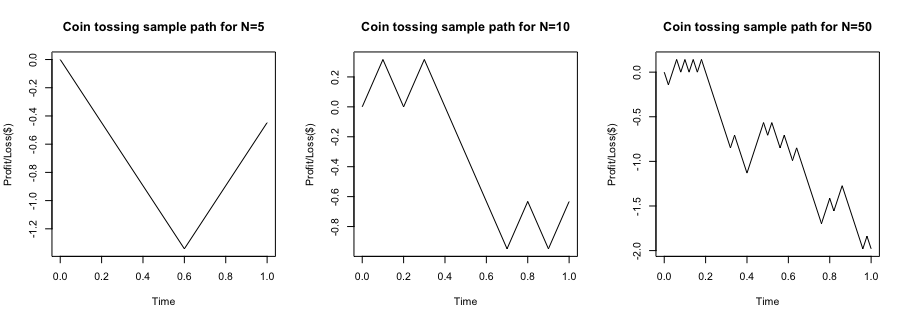
\includegraphics[scale=0.5]{plot1.png}
    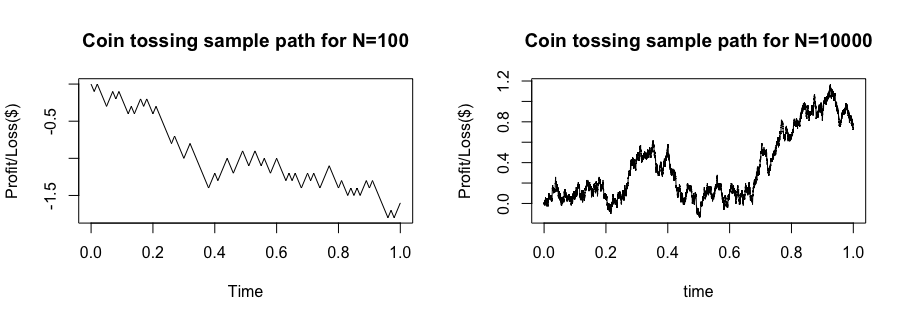
\includegraphics[scale=0.5]{plot2.png}
\end{figure}

En los gráficos podemos ver que, para valores de $N$ pequeños, por ejemplo $N=5$, el impacto de cada apuesta en la ganancia o pérdida total es relativamente grande, ya que el denominador es pequeño. Además, se esperan fluctuaciones más pronunciadas en la trayectoria, con cambios bruscos en la ganancia o pérdida en cada paso del tiempo. \\

A medida que $N$ va creciendo, por ejemplo para $N=10, 50$, el impacto de cada apuesta disminuye. La trayectoria del juego tiende a suavizarse, con fluctuaciones menos pronunciadas y cambios menos bruscos que en el caso anterior. \\

Finalmente, para valores de $N$ grandes, por ejemplo $N=100,10000$, el efecto de cada apuesta se vuelve aún más pequeño. 
La trayectoria del juego muestra una tendencia a comportarse de manera más suave y continua, esta vez, con cambios más graduales. \\

En resumen, a medida que aumenta $N$, el efecto de cada apuesta se atenúa, y la trayectoria del juego se vuelve más suave y menos volátil. \\

A continuación eestudiamos la distribución de las trayectorias generadas por la función anterior. Para ello creamos una función la cuál toma dos parámetros: $N$, que representa el número de apuestas en cada trayectoria, y $m$, que indica cuántas veces se ejecutará la simulación para obtener múltiples trayectorias. Esta función es:
% codi de la funció en R
\vspace{1cm}

Se puede ver que hemos utilizado la función anterior para generar múltiples trayectorias de juego, conservando el valor final de cada una. Estos valores finales se almacenan en un vector que representa la distribución de resultados después de realizar la simulación $m$ veces.\\

A continuación vamos a estudiar la distribución de beneficio acumulado para diferentes combinaciones de parámetros $(N, m)$, específicamente para los pares $(100,100), (1000,1000)$ y $(10000,10000)$. Las gráficas de su densidad son las siguientes
\begin{figure}[H]
    \centering
    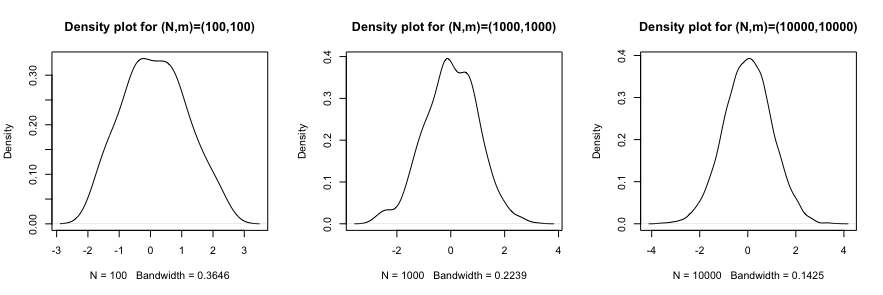
\includegraphics[width=1\linewidth]{plot3.png}  
\end{figure}
Podemos observar que, a simple vista, parecen seguir una distribución parecida a la distribución normal. Para poder afirmar este hecho hacemos una prueba de normalidad a cada par. Observamos que en todas las configuraciones obtenemos p-valores mayores que 0,05. \\

Así pues, tanto los gráficos de densidad como los tests de normalidad indican que, en estos casos, las distribuciones del beneficio acumulado tienden a seguir una distribución que se asemeja a la normal. \\

\section*{Ejercicio 2}

Queremos escribir una función que muestree una trayectoria de la ecuación diferencial estocástica de Black-Scholes
$$dS_t=rS_tdt+\sigma S_tdW_t$$
donde $S_t$ es el precio del activo subyacente en el momento $t$, $\sigma$ su volatilidad, $r$ el tipo de interés y $W_t$ un movimiento browniano. \\

Para ello, vamos a usar una discretización de Euler. Sabemos que, dada una ecuación diferencial estocástica general
$$dX_t=a(X_t)dt+b(X_t)dW_t$$
podemos simular el camino del proceso a partir de $[0,T]$ discretizando el intervalo de tiempo en $N$ pasos equidistantes ($0\leq t_0<t_1<\dotsb<t_n=T$). Al hacerlo obtenemos la llamada discretización de Euler, ésta es

\begin{equation*}
  \begin{cases}
    X_{t_0}&= x_0 \\
    X_{t+\Delta T} &= X_t+a(X_t)\Delta T+b(X_t)\sqrt{\Delta T}\epsilon_t,
\end{cases}  
\end{equation*}
donde $\epsilon_t\sim N(0,1)$ y $\Delta T=\frac{t_n-t_0}{N}.$ \\

Ahora, con el uso de esta última ecuación simularemos una trayectoria para los precios de las acciones suponiendo que
\begin{itemize}
    \item $S_{t_0}=S_0$
    \item $a(S)=rS$
    \item $b(S)=\sigma S.$
\end{itemize}

De este modo, la función que hemos creado es la siguiente:
% codi en R
\vspace{1cm}

Usando la función creada, queremos estudiar el par $(r, \sigma)$, donde vamos a ver cuáles son las propiedades de la trayectoria dependiendo de éste. Por ejemplo, si tomamos como valores iniciales $N=1000$, $t_0=0$, $t_n=1$, $S_0=100$, $r=0,01$, $\sigma=0,30$ obtenemos
\begin{figure}[H]
    \centering
    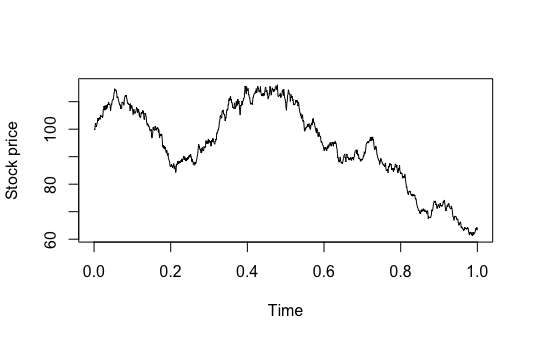
\includegraphics[width=0.6\linewidth]{plot4.png}
\end{figure}

Podemos ver que el valor de $\sigma$ controla la volatilidad de la serie temporal y el parámetro $r$ transforma la trayectoria muestral en una función casi lineal con comportamiento creciente cuando $0 < r \sim 1$. Por lo tanto, la tasa de interés $r$ determina la tendencia de la trayectoria y $\sigma $ su dispersión. Esta relación se ilustra de manera más clara en los gráficos siguientes.
\begin{figure}[H]
    \centering
    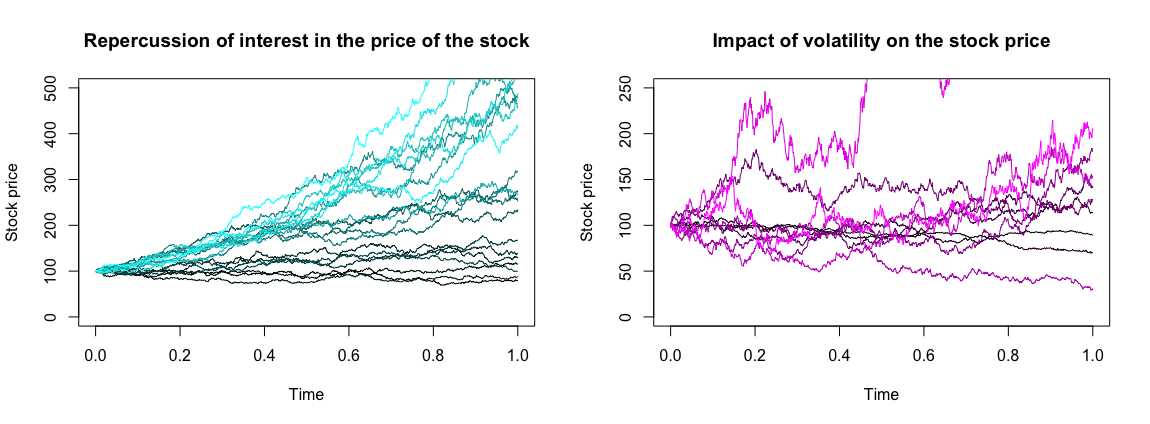
\includegraphics[width=1\linewidth]{plot5.png}
\end{figure}


Ahora, nuestro objetivo es implementar el algoritmo de Monte Carlo, para ello empezamos escribiendo la siguiente función \\
% codi de la funció
\vspace{1cm}

Ésta evalúa el pago de una opción CALL con un ejercicio $K$ determinado.\\

Iniciamos simulando una trayectoria para la variable $S$ mediante la discretización de Euler, siguiendo el mismo procedimiento que hemos utilizado previamente. Posteriormente, aplicamos la función de pago recién mencionada. Repetimos estos pasos un total de $M$ veces, registrando el resultado obtenido tras evaluar la función de pago en cada iteración y calculando su media. Al realizar este proceso, obtenemos el valor esperado del activo subyacente al momento del vencimiento. Dado que estamos interesados en determinar el precio de la opción en el día de hoy, necesitamos descontar este valor con la tasa de interés $r$ desde la fecha de vencimiento hasta el día actual. \\

Así pues, implementando el algoritmo de Monte Carlo, tenemos
% codi
\vspace{1cm}

Para acabar, vamos a modificar la función de pago de tal manera que nos proporcione el precio de una opción PUT a 1 año, con una tasa de interés del 5\% y una volatilidad del 40\%. Sabemos que la acción cotiza actualmente a 90 EUR y el ejercicio de la opción PUT es 75. \\

Nuestra función modificada es
%codi
\vspace{1cm}

y aplicando el método de Monte Carlo con la función de pago de una opción PUT y los datos dados, obtenemos un valor de 5.665408 EUR. Esto significa que la opción de venta en las condiciones indicadas debería tener un precio aproximado de 5,67 EUR. 

\end{document}
